\documentclass[a4paper]{report}
\usepackage[utf8]{inputenc}
\usepackage[]{amsmath}
\usepackage[]{braket} % \bra, \ket etc
\usepackage{graphicx}
\usepackage{tikz}
\usepackage{bm} % pour faire des vecteurs gras
\usepackage{subcaption} % package pour faire des subfigures
\usepackage{multirow} % package pour multirow/multicolumn
\usepackage{booktabs} % package pour top/mid/bottom rule
\usepackage{tcolorbox} % toujours plus de boites
\usetikzlibrary{optics}
\usetikzlibrary{shapes}
\usetikzlibrary{fit}

\title{Titre}
\author{Clément Pellet-Mary}
\date\today

\begin{document}
\chapter{L'atome}
  \section{Le moment cinétique}
  \subsection{Définition, relations de commutation}
  \textbf{Convention} : Dans tout ce chapitre, les vecteurs seront notés en \textbf{gras} et les opérateurs avec des chapeaux.
  
  En partant de la définition classique $\bm{L}=\bm{r} \times \bm{p}$ pour une particule, on obtient la version quantique avec la magie des chapeaux : \begin{equation}
  \hat{\bm{L}}=\hat{\bm{r}} \times \hat{ \bm p}
  \end{equation}
 Alors avec les relations de commutation sur $\hat{\bm{r}}$ et $\hat{ \bm p}$, on trouve : \begin{equation}
 [\hat L_x, \hat L_y]=i\hbar \hat L_z \quad , \quad [\hat L_y, \hat L_z]=i\hbar \hat L_x \quad , \quad [\hat L_z, \hat L_x]=i\hbar \hat L_y
 \end{equation}
 Qu'on peut également synthétiser en : \begin{equation}
 \hat{\bm L} \times \hat{\bm L} = i\hbar \hat{\bm L}
 \end{equation}
 C'est cette relation de commutation qu'on prendra comme définition d'un opérateur de moment cinétique, y compris quand $\bm{L}=\bm{r} \times \bm{p}$ n'existent pas (coucou le spin). Pour généraliser, on écrira $\hat{\bm J}$ pour un moment cinétique quelconque
 \subsection{Valeurs propres}
 On définit $\hat J^2= \hat J_x^2 + \hat J_y^2 + \hat J_z^2$. $ \hat J^2$ commute avec chacune des composantes de $\hat{\bm J}$ : \begin{equation}
 [\hat J^2, \hat{\bm J}]=0
\end{equation}  
(Composantes qui ne commutent pas entre elles, cf avant). 

On va alors former un ECOC à partir de $\hat{J^2}$ et d'une des trois composante qui sera par convention $\hat{J_z}$, c'est à dire que l'état du moment cinétique sera entièrement défini par la velur des deux nombres quantiques $j$ et $m$ sans dimension tels que :\begin{align}
\hat{J^2}\ket{j,m}&=j(j+1) \hbar^2 \ket{j,m} \\
\hat J_z\ket{j,m}&= m\hbar \ket{j,m}
\end{align}
$j$ est forcément positif car $\hat{J^2}$ est défini positif, et tu trouves que tu ne peux avoir que des valeurs demi-entières et que $-j \leq m \leq j$ par l'application répétée de $\hat L_\pm$ défini par :\begin{equation}
\hat L_\pm= \hat L_x \pm i \hat L_y
\end{equation}
Et qui vérifie :\begin{equation}
\hat L_\pm \ket{j,m} \propto \ket{j,m \pm 1}
\end{equation}
\subsection{Moment cinétique orbital et harmoniques sphériques}
On va maintenant s'intéresser à une particule ponctuelle qui a un moment cinétique classique. On peut donc bien écrire ici $\hat{\bm{L}}=\hat{\bm{r}} \times \hat{ \bm p}$

On se placera dans les coordonnées polaires habituelles ($r$,$\theta$,$\phi$) avec l'axe z comme axe polaire, $0 \leq \theta \leq \pi$ la colatitude en bon français et $0 \leq \phi \leq 2\pi$ l'angle azimutal.

Avec ces notations, en se rappelant que $\hat p_x = -i\hbar\dfrac{d}{dx}$ lorsqu'on raisonne en fonction d'onde, on trouve en coordonnées polaires : \begin{equation}
\hat L_z= -i\hbar \dfrac{d}{d\phi}
\end{equation}

Ce qui veut dire que les orbitales, c'est à dire les fonctions d'onde des états propres de $\hat L^2$ et $\hat L_z$, vérifient : \begin{equation}
\hat L_z \psi_{lm}(r,\theta, \phi)= -i\hbar \dfrac{d}{d\phi} \psi_{lm}(r,\theta, \phi) = \hbar m \psi_{lm}(r,\theta, \phi)
\end{equation}
D'où : \begin{equation}
\psi_{lm}(r,\theta, \phi)= \varphi(r,\theta)e^{i m \phi}
\end{equation}

Puisqu'une rotation de $\phi$ de $2\pi$ doit donner la même fonction d'onde (? pourquoi c'est pas vrai sur la sphère de Bloch, parce que ce n'est pas l'espace physique ?), on en déduit que \textbf{m et don l sont nécessairement entiers}

C'est également vrai pour $\hat L^2$ mais sa formule est plus dégueu : \begin{equation}
\hat L^2= -\hbar ^2 \left( \dfrac{1}{\sin \theta}\dfrac{d}{d\theta}\sin \theta\dfrac{d}{d\theta}+ \dfrac{1}{\sin ^2 \theta} \dfrac{d}{d\phi} \right)
\end{equation}

En faite c'est la partie angulaire du laplacien sphérique : \begin{equation}
\Delta = \dfrac{1}{r}\dfrac{d^2}{dr^2}-\dfrac{1}{r^2\hbar^2}\hat L^2
\end{equation}

On constate également que $\hat L^2$ et $\hat L_z$ n'agissent pas sur la partie radiale de l'orbitale, on va donc décomposer l'orbitale en sa partie radiale et sphérique : \begin{equation}
\psi_{lm}(r,\theta,\phi)=R_{l}(r)Y_{lm}(\theta,\phi)
\end{equation}
Où les $Y_{lm}$ sont les \textbf{Harmoniques sphériques}, c'est à dire les fonction propres de $\hat L^2$ et $\hat L_z$ normalisées à 1.

On remarque que $L_z$ n'agit pas sur la partie radiale de $\psi_lm$, d'où le fait que $R_{l}$ ne dépendent pas de $m$

\subsection{Lien avec le moment magnétique}
Toute particule chargée avec un moment cinétique (orbital ou non) dispose également d'un moment magnétique.

Pour rappel, l'interaction d'un moment magnétique avec un champ s'écrit : \begin{align}
W &= - \bm \mu \cdot \bm B \\
\bm \Gamma &= \bm \mu \times \bm B
\end{align}
\subsubsection{Pour un moment cinétique orbital}
Analogie classique : tu as une spire de courant formée par ta particule et son mouvement (circulaire ici mais je crois que c'est général) :
\begin{align}
\bm L &= \bm r \times \bm p = m_q r v \bm u \\
\bm \mu &= I S \bm u = \dfrac{qv}{2\pi r}\pi r^2 \bm u = \dfrac{q}{2} v r \bm u
\end{align}
D'où : \begin{equation}
\bm \mu = \gamma_0 \bm L \quad \mathrm{avec} \quad \gamma_0=\dfrac{q}{2 m_q}
\end{equation}
\emph{note :} $q$ est algébrique, dans le cas de l'électron $q=-e$

$\gamma_0$ est appelé le \textbf{rapport gyromagnétique} de ta particule. \\

On définit également le \textbf{magnéton de Bohr} comme le quanta de moment magnétique (du au mouvement orbital) pour l'électron : 
\begin{equation}
\mu_B=\gamma_0 \hbar= -\dfrac{q \hbar}{2 m_e}
\end{equation}
\subsubsection{Pour un moment cinétique intrinsèque}
De la même façon, on postule (je crois pas qu'il y ait de preuve, si ce n'est expérimentale) que les moments cinétiques intrinsèques sont proportionnels à un moment magnétique.

On doit quand même introduire un facteur sans dimension supplémentaire par rapport au moment cinétique orbital : le \textbf{facteur de Landée $g$} : \begin{equation}
\bm \mu_s= g\dfrac{q}{2m_q} \bm J
\end{equation}

Les valeurs numériques de g sont : \begin{align*}
\mathrm{electron} &\approx -2.00 \\
\mathrm{proton} &\approx +5.59 \\
\mathrm{neutron} &\approx -3.83
\end{align*}

\subsection{Composition de moments cinétiques}
\begin{figure}[h]
\centering

\includegraphics[width=.5\linewidth]{Clebs_Jordan.jpg}
\caption{Clebs-Jordan, le cousin de Clebsch-Gordan}
\end{figure}
Ça peut concerner deux particules en interaction ou un moment orbital et un moment intrinsèque. On va donc considérer deux moments : $\hat{\bm J_1}$ et $\hat{\bm J_1}$

Dans la base découplée, ton système est donc décrit par les 4 nombres quantiques naturels : $\ket{j_1,m_j,j_2,m_2}$.

Cependant on constate que $\hat{\bm J}=\hat{\bm J_1}+\hat{\bm J_2}$ est également un moment cinétique, on peut alors former un nouvel ECOC avec les 4 observables : $\hat J^2, \hat J_z, \hat J_1^2$ et $\hat J_2^2$. Les 4 nouveaux nombres quantiques de la base couplée seront donc : $\ket{j,m,j_1,j_2}$.

Il y a deux avantages à passer dans la base couplée : 
\begin{itemize}
\item D'une part dans le cas de moment cinétiques orbitaux, $J$ représente bien le moment cinétique total du système
\item D'autre part dans le cas d'une interaction, tu vas très souvent te retrouver (au premier ordre) avec un terme dans le hamiltonien en $\hat{\bm J_1} \cdot \hat{\bm J_2}$. Or $\hat{\bm J_1} \cdot \hat{\bm J_2}= \dfrac{1}{2}(\hat J^2- \hat J_1^2 - \hat J_2^2$ (source : mon cours de troisième). Donc les états de la base couplée sont états propres du Hamiltonien, et ça c'est toujours sympathique.
\end{itemize}

\subsubsection{Passage d'une base à l'autre}

Dans la théorie tu utilises $J^-=J_1^-+J_2^-$ en partant de l'état $m=j$ qui est présent dans les deux bases, dans la pratique tu regardes les coefs de Clebsch-Gordon : 

\begin{center}
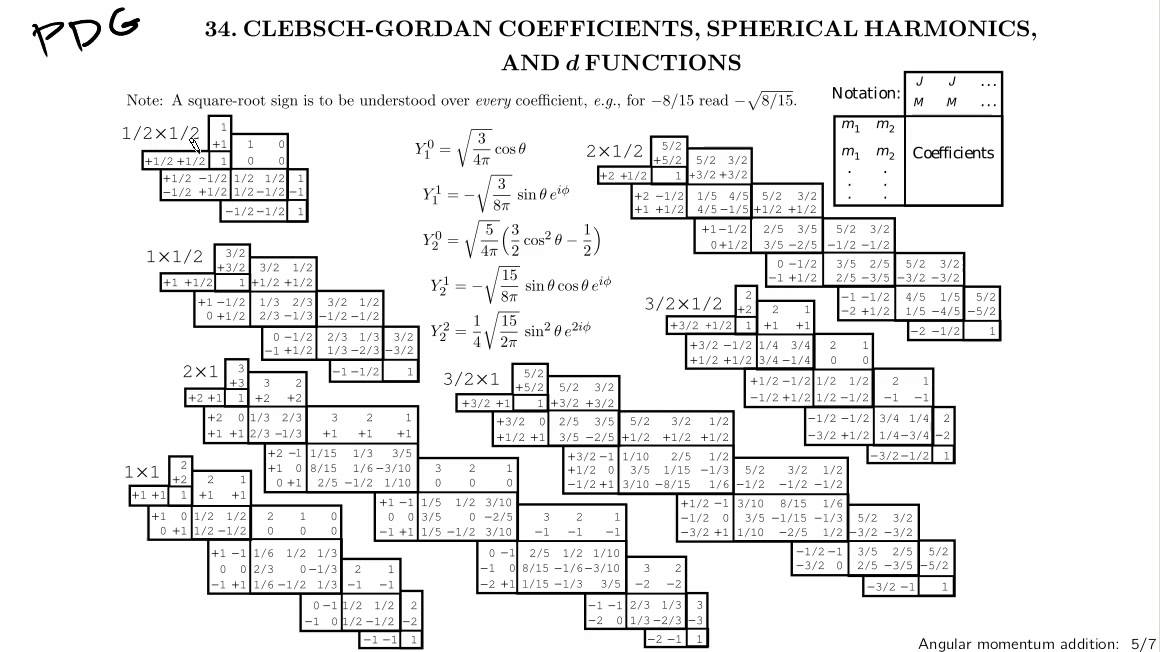
\includegraphics[scale=.35]{Clebsch_Gordan}
\end{center}

(je sais c'est écrit petit, mais c'est ces vicieux de la physique des particules).

Dans tous les cas tu constates que $\hat J_1^2$ et $\hat J_2^2$ sont présents dans les deux bases donc tu n'as que 2 nombres quantiques à changer.

\subsection{Lois de conservations}

Pour la projection c'est très clair, vu que $m=m_1+m_2$. Le moment total c'est plus compliqué vu qu'il y a la conservation de l'énergie qui s'en mêle.

\section{Nombres quantiques d'un état atomique}
Dans toute cette partie on s’intéresse à l'atome d'hydrogène. Ça se généralise assez bien aux alcalins mais tout le reste c'est plus compliqué.
\subsection{Hamiltonien}
Dans l'absolu c'est le problème à deux corps, que tu sépare en une partie avec les coordonnées du centre de masse, et une partie avec les coordonnées relatives. Dans la pratique on va considérer l'électron dans un potentiel central généré par le proton immobile dans le référentiel du labo, parce qu'il y a un rapport 2000 entre les masses. De toute façon les calculs sont identiques.

\begin{equation}
H=\dfrac{p^2}{2m}+V(r)
\end{equation}

On s’intéresse aux solutions stables, donc ESIT : \begin{equation}
\Delta \psi (\bm r) + V(r) \psi (\bm r) = E \psi (\bm r)
\end{equation}

Avec la définition du laplacien sphérique en fonction de $\hat L^2$ et la décomposition en harmonique sphérique $\psi_{lm}(r,\theta,\phi)=R_{l}(r)Y_{lm}(\theta,\phi)$, on trouve finalement une EDO sur $R_l$ : \begin{equation}
\left(-\dfrac{\hbar^2}{2m}\dfrac{1}{r}\dfrac{d^2}{dr^2}r + \dfrac{l(l+1)\hbar^2}{2mr^2} + V(r) \right) R_l(r) = E R_l(r)
\end{equation} \\


\textbf{Remarque} : C'est parce que $\hat H$, c'est à dire $\hat V$, commute avec $L_z$ et $L^2$ que tu peux décomposer les solutions comme ça. Et c'est vrai ici parce que V est invariant selon $\theta$ et $\phi$.
\subsection{Solutions de l'ESIT}

Bon en vrai c'est un peu chaud les solutions de l'EDO, ce qu'on peut retenir c'est que : \begin{itemize}
\item Comme pour tout système lié, il y a discrétisation des $E<0$ possibles
\item Pour un $l$ donné, il n'existe qu'une solution pour chaque valeur propre $E_{n'}$ donnée. On peut donc définir sans équivoque $\ket{l,n'}$
\item La partie radiale de la fonction d'onde $R_{n'l}(r)$ a exactement $n'$ zéros.
\item L'énergie $E_{n'l}$ correspondante est \begin{equation}
E_{n'l}=-\dfrac{E_0}{(n'+l+1)^2}
\end{equation}
Avec $E_0$ l'énergie du fondamental, c'est à dire l'énergie d'ionisation de l'atome d'hydrogène, c'est à dire un Ryldberg (techniquement les Ry c'est en $\mathrm{cm}^{-1}$ je crois) : \begin{equation}
E_0=\dfrac{m_e e^4}{2\hbar^2}\approx13.6 \mathrm{eV}
\end{equation}
\item A cause de l'expression de l'énergie, on utilise comme nombre quantique \begin{equation}
n=n'+l+1
\end{equation}  Donc maintenant l'énergie peut ne s'exprimer qu'en fonction de $n$, mais elle dépend quand même de $l$. Bref en vrai ça complique la vie plus qu'autre chose.
\end{itemize}
\subsection{Notations spectro}
Bon je t'épargne l'histoire (c'est à cause des séries de raies de l'atome d'hydrogène : sharp, principal, diffuse...) mais 3d $\Rightarrow n=3\; \mathrm{et} \;l=2$
\subsection{Solutions particulières}
\subsubsection{Orbitale 1s}
$l=0$ et $n'=0$, $Y_{l,m}(\theta, \phi)=1/\sqrt{4\pi}$, ta fonction est : \begin{equation}
\psi_{1,0,0}(\bm r) = \dfrac{e^{-r/a_0}}{\sqrt{\pi a_0^3}}
\end{equation}
\textbf{note :} pour tout $n'$ tu es dominé aux grands $r$ par un $e^{-r}$. \\

Si on s'intéresse à la densité de présence radiale, il faut intégrer sur une sphère de rayon $r$, d'où :
\begin{equation}
\rho(r)=|\psi_{1,0,0}(\bm r)|^2 4 \pi r^2= e^{-2r/a_0} \dfrac{r^2}{a_0^3}
\end{equation}

Et on constate que $<r> = a_0$, la distance moyenne de l'électron est bien le rayon de Bohr

\subsubsection{Orbitale 2s}
Toujours une symétrie sphérique car $l=0$, mais cette fois ci ta fonction s'annule et change de signe en $r=a_0/2$. Tu as donc une région interdite pour ton électron. \begin{equation}
\psi_{2,0,0}(\bm r) \propto \left(1-\dfrac{r}{2 a_0}\right) e^{-r/a0}
\end{equation}

\subsubsection{Orbitale 2p}
Ici on commence les embrouilles car $l=1$ et donc $m$ commence à prendre des valeurs non nulles. En plus $p_x$ et $p_y$ c'est des c.l des états propres (ils ne sont donc pas état propre de $L_z$, ce qui est plutôt logique vu que c'est les états propres de $L_x$ et $L_y$).

\begin{align}
\psi_{pz}(\bm r) &\propto Y_{1,0}(\theta,\phi) e^{-r/a_0} \propto \cos \theta  e^{-r/a_0} \\
\psi_{px}(\bm r) &\propto (Y_{1,1}+Y_{1,-1})(\theta,\phi) e^{-r/a_0} \propto \sin \theta \sin \phi e^{-r/a_0} \\
\psi_{py}(\bm r) &\propto (Y_{1,1}-Y_{1,-1})(\theta,\phi) e^{-r/a_0} \propto \sin \theta \cos \phi e^{-r/a_0}
\end{align}

\subsection{Et le spin dans tout ça}
Ton système c'est un électron, donc $s=1/2$ on ne le note pas. Sa projection $m_s=\pm 1/2$ n'influe ni sur les niveaux d'énergie (sans champ magnétique), ni sur les orbitales. En revanche ça joue sur la population des états.

\section{Modification des niveaux d'énergie}
\subsection{Couplage spin-orbite : structure fine}
\subsection{Effet Zeeman}
\subsection{Effet Stark}
\subsection{Couplage spin-spin : structure hyper-fine}
\subsection{Quantification du champ : Lamb shift}

  \end{document}	
  
  